\section{Corpo macchina e fisionomia di una reflex} \label{sec:fisionomia}

Quando scattiamo una foto abbiamo in mano un \textbf{corpo macchina} con attaccato un \textbf{obiettivo}; spesso, per comodità, usiamo il termine \textit{macchina fotografica} per indicare il tutto, e di per sé, visto l'ampio utilizzo di questo modo di dire, non è sbagliato, ma è bene sapere che la macchina fotografia, in teoria, è solo il corpo macchina.

Esistono diversi tipi di corpi macchina, oggi i più diffusi sono:
\begin{itemize}
    \item[-] \nameref{subsec:dslr}
    \item[-] \nameref{subsec:mirrorless}
\end{itemize}


\subsection{DSLR} \label{subsec:dslr}
DSLR sta per \textbf{Digital Single Lens Reflex}.\newline
Il nome indica una fotocamera reflex, a lente singola e digitale. Se parliamo di una fotocamera analogica si chiama semplicemente \textbf{SLR}, non è digitale e quindi la D iniziale non c'è.

Vediamo cosa c'è dentro il corpo macchina, per capire bene cosa c'è dentro una macchinetta, cosa vediamo e in che senso è una \textit{reflex} (i.e. riflesso).

\setlength{\columnsep}{2.8cm}
\begin{multicols}{2}
    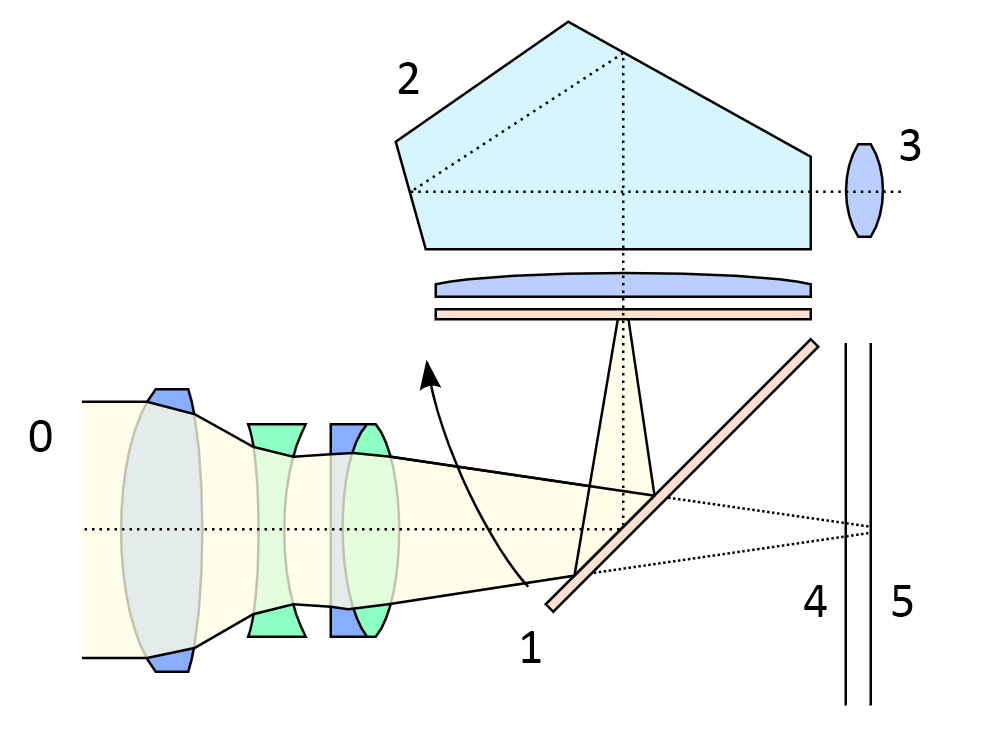
\includegraphics[width=0.66\textwidth]{Reflex.png}

    \columnbreak

    \begin{enumerate}
        \setcounter{enumi}{0}
        \item Obiettivo
        \item Specchio a 45º
        \item Pentaprisma
        \item Mirino
        \item Otturatore
        \item Sensore
    \end{enumerate}
\end{multicols}

La luce segue il percorso indicato dalla linea a puntini.\newline
L'\textit{obiettivo} fa entrare la luce, che rimbalza sullo \textit{specchio a 45º} ed entra nel \textit{pentaprisma}; una volta nel \textit{pentaprisma} la luce fa un paio di rimbalzi e torna a seguire il verso iniziale, entra nel \textit{mirino}, dove mettiamo noi l'occhio per vedere \textit{esattamente} cosa vede l'obiettivo.

Notiamo come la luce non ha modo di arrivare al sensore, cosa succede quando viene scattata una foto?\newline
Come prima cosa lo \textit{specchio a 45º} si alza (seguendo la freccia nell'immagine), in questo modo noi dal \textit{mirino} vedremo tutto nero, mentre la luce ha modo di arrivare direttamente sull'\textit{otturatore}.
L'\textit{otturatore} è una tendina che a questo punto si apre (per il tempo di scatto da noi impostato) e fa sì che la luce colpisca il sensore e la foto venga catturata.

Una volta passato il tempo di scatto la tendina (i.e. l'\textit{otturatore}) si richiude e lo \textit{specchio a 45º} torna giù.

Le fotocamere hanno una modalità chiamata \textit{Live view}, che ci permette di vedere direttamente cosa sta guardando il sensore. Quando attiviamo il Live view lo specchio a 45º si alza e rimane bloccato, non è più possibile usare il mirino per inquadrare ma dobbiamo usare lo schermo della fotocamera. A che pro usare la modalità live view?

Un problema dei mirini, specialmente quelli sulle fotocamere di fascia più bassa, è che non coprono tutta la porzione del sensore, nel senso che i bordi più estremi di quello che vede il sensore non si vedono dal mirino.
Usare lo schermo permette inoltre si poter mettere a fuoco con grande precisione e di vedere in anticipo come sarà l'immagine (i.e. un anteprima di come l'immagine sarà esposta).

Che problemi ha invece il live view? Oltre ad una soggettiva questione di preferenze (può non essere sempre comodo per tutti usare lo schermo) avere il sensore sempre attivo consuma più batteria e lo riscalda; in situazioni normali non c'è il pericolo che con il live view il sensore si surriscaldi, ma certamente tenerlo sempre attivo ne alza le temperature.
\footnote{Nota dell'autore: non penso di aver mai letto del problema del sensore che si riscalda in live view, sebbene sono sicuro sia vero che succeda sono anche sicuro che si riscaldi talmente poco da non poterlo neanche definire un problema; è bene però specificare che è un mia "intuizione" e che non ho mai letto studi a riguardo}


\subsection{Mirrorless} \label{subsec:mirrorless}
Sono fotocamere che hanno preso piede negli ultimi anni. Una mirrorless è, a grandi linee, simile ad una reflex, ma con la fondamentale differenza che non c'è l'aspetto della luce riflessa (i.e. reflex), manca tutto il meccanismo con lo specchio a 45º e il pentaprisma, la luce arriva direttamente al sensore e per vedere cosa stia vedendo il sensore si può usare soltanto lo schermo.

A che pro usare una mirrorless? La mancanza del meccanismo di specchi fa sì che le mirrorless siano più piccole e leggere, inoltre gli specchi hanno un grande difetto: dovendo muoversi fanno rumore, e in certe situazioni possono
causare dei micromovimenti del corpo macchina che si vanno poi a ripercuitere sulla foto (i.e. sulla foto esce fuori del \textbf{micromosso}).\newline
L'assenza degli specchi permette anche di avere l'obiettivo più vicino al sensore, a giovamento della qualità della foto.

Che problemi possono avere quindi le mirrorless? Abbiamo visto che sulle DSLR la modalità live view consuma molta batteria, tenere costantemente il sensore attivo per inviare il segnale al sensore costa e non poco, le mirrorless è proprio su questo che si basano, sono in costante modalità live view. Ecco quindi il loro difetto, forse, più importante: una scarsa durata della batteria. Si consiglia infatti, a chi acquista una mirrorless, di comprare almeno 1-2 batterie di scorta.

Può capire di vedere qualche modello di mirrorless con un mirino, in quei casi dentro il mirino non c'è altro che un mini schermo, che mostrerà l'immagine vista dal sensore, esattamente come lo schermo sul retro della fotocamera.
A che serve quindi? Come accennato in precedenza (vedi \nameref{subsec:dslr}) questione di preferenze, c'è chi preferisce guardare dentro il mirino piuttosto che tenere la fotocamera davanti a sé per guardare lo schermo.

Un vantaggio, meno banale di quanto si possa pensare, di usare il mirino piuttosto che lo schermo, è che col mirino teniamo la fotocamera molto vicina al nostro corpo, con lo schermo invece la dobbiamo spostare in avanti, e sulle lunghe si stancano di più spalle e braccia. Le fotocamere, se parliamo di DSLR e mirrorless non pesano molto, i modelli più estremi superano non di molto 1kg, il problema sono gli obiettivi: possono superare tranquillamente i 2-3kg, specialmente se abbiamo tra le mani un obiettivo più datato fatto di metallo e non di plastica.
Va però anche detto che gli obiettivi più pesanti sono solitamente teleobiettivi molto lunghi, per i quali è consigliabile in ogni caso usare un treppiedi, a quel punto tutto il discorso del peso non vale più.